\subsection{Metaheuristics}

\subsubsection{Definition}
~\\
~\\
The $meta$ and $heuristic$ are Greek words, $meta$ it means $higher level$ and $heuristics$ means $to$ $find$, $to$ $know$ or $to$ $discover$. Metaheuristics are a set of intelligent strategies to enhance the efficiency of heuristic procedures.\\
A metaheuristic will be successful on a given optimizaction problem if it can provide a balance between exploration and exploitation. Exploration means to generate diverse solutions so as to explore the search space on the global scale, while exploitation means search in a local region by exploiting the information that a current good solution is found in this region.
exploration, often by use of randomization, which enables an algorithm to have the ability to jump out of any local optimum so as to explore the search globally.

\subsubsection{Clasification}
~\\
~\\
The different metaheuristic approaches can be characterized by different aspects concerning the search path they follow or how memory is exploited \cite{citeulike:1859945}. A majority of these algorithms has a stochastic behavior and mimics biological or  physical processes. The classification presented was proposed by Beheshti et al. \cite{Beheshti:2014:CCA:2563733.2564085}, and can be understood better as shown in the (Figure \ref{fig:classification-of-mh}).

\squeezeup
\begin{figure}[ht]
	\centering
  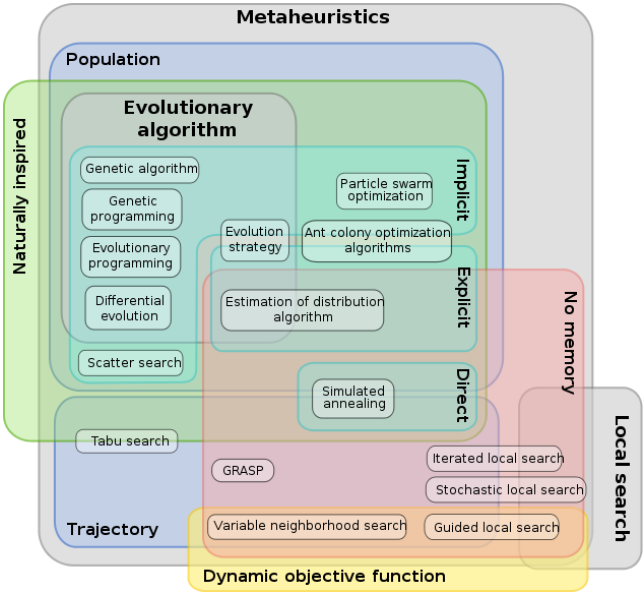
\includegraphics[width=0.70\textwidth]{MarcoTeorico/imagenes/classification_mh.png}
	\caption{Classification of metaheuristic}\label{fig:classification-of-mh}
\end{figure}
\squeezeup


~\\
\textbf{Nature-inspired vs. non-nature inspiration }
This class is based on the origin of algorithm. The majority of meta-heuristics are nature-inspired algorithms such as Black Hole (BH) \cite{Rubio2016}, Particle Swarm Optimization (PSO) \cite{Duran:2010:CPS:1645454.1645859} and Genetic Algorithms (GA) \cite{DBLP:conf/icsi/CrawfordSPJPO14}. Also, some of them are non-nature-inspired algorithms like Iterated Local Search (ILS) \cite{DBLP:journals/networks/AringhieriGHS16} and TabuSearch (TS) \cite{DBLP:journals/eswa/SotoCGMP13}.

~\\
\textbf{Population-based vs. single-point search}
There is a certain group of metaheuristics, which can be classified by the number of solutions in the lifecycle or execution, such as Trajectory methods, which are the algorithms working based on a single solution at any time (Figure \ref{fig:trajectory-method}). On the other hand Population-based algorithms perform search with multiple initial points in a parallel style. Examples of these metaheuristics can be: Harmony Search (HS) \cite{DBLP:conf/ccece/Al-AjmiE14}, GA \cite{Aupetit2008} and PSO. 

\squeezeup
\begin{figure}[H]
	\centering
  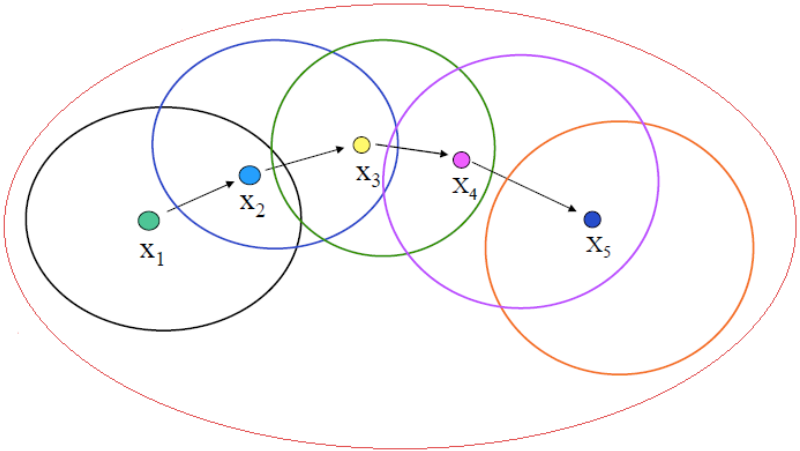
\includegraphics[width=0.55\textwidth]{MarcoTeorico/imagenes/trajectory-mh.png}
	\caption{Trajectory-based method}\label{fig:trajectory-method}
\end{figure}
\squeezeup

~\\
\textbf{Dynamic vs. static objective function}
Another way of classifying metaheuristics, is by the way of utilizing the objective function, some algorithms maintain the objective function intact throughout the execution cycle, while others modify the objective function according to information collected at runtime.\\
An example of the second case presented, is Guided Local Search (GLS) \cite{DBLP:journals/eor/VansteenwegenSBO09}.  The idea behind this approach is to escape from local optima by changing the search landscape. 

~\\
\textbf{One vs. various neighborhood structures}
The majority of metaheuristic algorithms apply one single neighborhood structure. The fitness landscape topology does not alter in the course of the algorithm while others, like Variable Neighborhood Search (VNS) \cite{DBLP:journals/anor/SarasolaDSA16}, employ a set of neighborhood structures. This latter structure gives the possibility to diversify the search by swapping between different fitness landscapes.

~\\
\textbf{Memory usage vs. memoryless methods}
One of the most interesting variables to classify a metaheuristic is undoubtedly use of memory. Short term usually is different from long term memory. The first kind usually keeps track of recently performed moves, or decisions taken. The second is usually an accumulation of synthetic parameters about the search. 

\subsubsection{Related terms}
~\\~\\
\textbf{Operator:} 
Unitary procedure for transforming information or implement the behavior of the algrithm.

~\\~\\
\textbf{Solution:} 
Array of $n$ columns containing a solution for a given problem. In the binary case, the posible values are $0$ and $1$.

~\\~\\
\textbf{Constrain:} 
Conditions to be met to find a viable solution.

~\\~\\
\textbf{Benchmark:} 
Optimal set of known problem instances to validate the propose algorithm.

~\\~\\
\textbf{Objective Function:}  
Implements the mathematical expression representing the problem to solve. The guiding objective function is related to the goal to achieve.

~\\~\\
\textbf{Fitness:} 
Value resulting by applying the objective function to solution.

~\\~\\
\textbf{Matrix of Costs:} 
Consist of $n$ columns vector containing the cost associated with each problem variable.

~\\~\\
\textbf{Optimal Value:} 
Solution with the best fitness.

~\\~\\
\textbf{Domain:} 
Set of possible values for the variable.

~\\~\\
\textbf{Matrix A:} 
Matrix containing the restrictions for the given problem.

~\\~\\
\textbf{RPD:} 
Relative Percentage Deviation.

~\\~\\
\textbf{Harmony Memory:} 
Memory space which includes the population of the solution vectors.

~\\~\\
\textbf{Harmony Memory Size:} 
Defines the amount of harmonies that can be stored in HM.

~\\~\\
\textbf{Harmony Memory Consideration Rate (HMCR):} 
In memory consideration, the value of decision variable ${x\textprime}_1$ is randomly selected from the historical values, other decision variables, $({x\textprime}_2, {x\textprime}_3,\dots,{x\textprime}_N)$ are sequentially selected in the same manner with probability where HMCR $\in$ (0,1).

~\\~\\
\textbf{Pitch Adjusting Rate (PAR):} 
Each decision variable ${x\textprime}_i$ assigned a value by memory considerations is pitch adjusted with the probability of PAR where PAR $\in$ (0,1).

\subsubsection{Framework for development}
In an effort to maintain consistency in the structure of the proposed metaheuristic development, a well-defined model is followed, in order to structure the development steps of the proposed technique (Figure \ref{fig:GuideSolvingSCP}). \\
~\\
The first step consists in modeling the problem and also define application requirements. In the particular case of this investigation the SCP is defined and it is validated against instances of benchmarck. the number of iterations but not the runtime is considered.\\

The second step basically corresponds to design metaheuristic. In the case of this research, we will work with variants of Harmony Search. That is to say not designed from the ground up, but certain elements that make the behavior of the technical improvement in some aspects be incorporated. Given the nature of the problem to be solved and metaheuristic to use. Elements like the objective function to use and classification (Population based) are set by default.\\

The third step is to adopt a strategy of development of the technique or metaheuristic. In this research, we chose to develop metaheruistica from scratch, thereby achieving maximum control of it. It was used for this purpose Python 2.7 as programming language and  PyCharm as IDE.\\

The fourth step is handling optimization parameters. There are two types of parameter tuning, Online and Off line. In this research, management of both types is performed to achieve good results. Specifically improving the metaheuristic proposal is based on the dynamic variation of the parameter that generates solutions. The following sections will go into detail on this subject.\\

The fifth and final step is to design experiments, get results and compare improvements. Then perform changes in parameters or operators so as to keep improving convergence, achieving an optimum balance between exploration and exploitation. This framework adopts an iterative approach because when step five is completed, you can return to step one, two or three to seek a better solution.







